\documentclass{report}

\usepackage{phdstyle}
\usepackage{RepSty}

\usepackage{setspace}

\usepackage[numbers]{natbib}

\newcommand{\home}{\string~}
\newcommand{\Artem}{\home/REPOS/COSYINF/img/Artem}
\newcommand{\multisext}{\Artem/multisext_test}
\newcommand{\compare}{\Artem/spin_vs_polarization_fit_comp}
\newcommand{\decoh}{\Artem/decoherence_frequency_dependence}

\begin{document}
\singlespacing
\begin{titlepage}

\begin{center}
{МИНИСТЕРСТВО ОБРАЗОВАНИЯ И НАУКИ РОССИЙСКОЙ ФЕДЕРАЦИИ}\\[3pt]
\textsc{\small{Федеральное государственное автономное образовательное учреждение высшего образования}}\\

\textbf{\enquote{Национальный исследовательский ядерный университет\\
{``МИФИ''}}}\\
\textbf{(НИЯУ МИФИ)}\\[2cm]




\textsc{\textbf{Отчет о научной практике,\\		
		проводимой в рамках диссертационного исследования}}\\[2cm]

% Title
\enquote{Исследование магнитооптических структур со свойствами замороженного и квази-замороженного спина для поиска электрического дипольного момента дейтрона в накопительном кольце}\\[2cm]

\textsc{\textbf{4 курс}}\\[2cm]


\end{center}


\begin{flushleft}
% Author and supervisor
\begin{tabular}{ll}
	Аспирант                   & А.Е. Аксентьев                           \\
	Направление                & 03.06.01 Физика и астрономия             \\
	Научная специальность      & 01.04.20 Физика пучков заряженных частиц \\
	                           & \-\hspace{1.8cm} и ускорительная техника \\[1cm]
	Научный руководитель       &                                          \\
	Должность, степень, звание & С.М. Полозов, к.ф.-м.н, доц.             \\%[1cm]
	                           & Ю.В. Сеничев, д.ф-м.н., проф.            \\[1cm]
	Дата защиты:               &                                          \\
	Результат защиты:          &
\end{tabular}

\end{flushleft}

\vfill


\begin{center}
Москва \the\year{}
\end{center}



\end{titlepage}


\tableofcontents 
\pagebreak

\onehalfspacing

\chapter{Теоретическая основа экспериментов по поиску Электронного Дипольного Момента элементарных частиц}
\newcommand{\dotprod}[2]{\; {#1} \cdot {#2}\;}
\newcommand{\xprod}[2]{{#1} \times {#2}}
\newcommand{\tensprod}[2]{#1 \otimes #2}
\newcommand{\SMatrix}{\mathcal{S}}
\newcommand{\TMatrix}{\mathcal{T}}
\newcommand{\IMatrix}{\mathcal{I}}

\newcommand{\ampl}[2]{\langle #1 \vert #2 \rangle}
\newcommand{\ket}[1]{\vert{#1}\rangle}
\newcommand{\bra}[1]{\langle{#1}\vert}

\section{Барионная Асимметрия} 

В соответствии с теорией Большого Взрыва, при рождении Вселенной, материя и антиматерия должны были быть произведены в равных количествах: на каждый кварк -- антикварк, на каждый электрон -- позитрон и т.д., что является следствием симметричности физических законов данной теории.

Тем не менее, вся наблюдаемая вселенная состоит исключительно из материи; антиматерия может быть получена в ускорителе заряженных частиц, но в количествах, пренебрежимо малых по сравнению с материей.

Решением этого парадокса может быть асимметрия физических законов в сторону производства материи, что в Стандартной Модели (СМ) элементарных частиц может быть выражено нарушением фундаментальных симметрий. В 1967 году, академик АН СССР Андрей Сахаров сформулировал три условия бариогенеза:~\cite{Perepelitsa:Baryogenesis}
\begin{enumerate}
\item В начале эволюции вселенной, должен был существовать по крайней мере один процесс, нарушающий сохранение числа барионов,
\item необходимо нарушение С- и CP-симметрий,
\item генерация барионов должна была происходить при нарушении температурного равновесия.
\end{enumerate}


\section{Симметрии в природе}
В Стандартной Модели элементарных частиц рассматриваются три типа фундаментальных симметрий:~\cite{Sozzi:Symmetries}
\begin{enumerate}
\item C-симметрия (зарядовая): уравнения физических процессов не меняются при смене знаков зарядов на противоположные;
\item P-симметрия (чётность): инвариантность уравнений относительно смены знаков координат всех частиц на противоположные;
\item T-симметрия (время): инвариантность уравнений относительно замены времени с $+t$ на $-t$.
\end{enumerate}

В 1954 году, Г. Людерс и В. Паули, независимо друг от друга, доказали CPT-теорему: во всех процессах квантовой теории поля сохраняется CPT-симметрия. Следствием этого является то, что нарушение CP-симметрии влечёт за собой нарушение T-симметрии, и наоборот.~\cite{Luders:CPT},~\cite{Pauli:CPT}


\section{Электрический Дипольный Момент (ЭДМ)}

Электрическим диполем называют систему из двух противоположных зарядов $\pm q$, разделённых расстоянием $d$. Электрический дипольный момент (ЭДМ) двух точечных зарядов определяется выражением $p = qd$.

ЭДМ заряда, распределённого с плотностью $\rho(\vec r)$ в объёме $V$, равен
\[
p(\vec r) = \int_V\rho(\vec r_0)(\vec r_0-\vec r)\rd^3\vec r.
\]

Если полный заряд $Q$ в объёме $V$ равен нулю, ЭДМ $p(\vec r)$ не зависит от точки отсчёта. Для заряженных частиц, $Q\neq0$, и ЭДМ определяется в системе их центра масс.~\cite[стр.~2]{Eremey:Thesis}

Существование ненулевого ЭДМ фундаментальной частицы нарушает и C- и CP- симметрии,~\cite{Ramsey:EDM} а значит свидетельствует в пользу условий бариогенеза Сахарова. До настоящего времени, ЭДМ элементарных частиц не наблюдался экспериментально. Порядок ЭДМ нейтрона, совместимый с СМ, находится на уровне $10^{-32} < |d_n| < 10^{-31}~e\cdot cm$.~\cite{Khriplovich:EDM} В то же время, теории за пределами СМ, такие как SUSY, предсказывают существование ЭДМ нейтрона в пределах $10^{-29} < |d_n| < 10^{-24}~e\cdot cm$.~\cite{JEDI:Intro}

\chapter{Описание эксперимента}
Методология Frequency Domain была предложена в рамках коллаборации JEDI Исследовательского центра ``Юлих'' проф. Ю. Сеничевым. Она предполагает инжекцию продольно-поляризованного пучка в состоянии ``замороженного спина'' в комбинированное накопительное кольцо, и измерение частоты прецессии его поляризации в вертикальной плоскости. Измерение частоты производится при движении пучка по часовой стрелке, а затем против часовой. Измеренные частоты содержат в себе вклады (с одним знаком) от ЭДМ, а также от МДМ (с противоположными знаками); при их сложении МДМ эффект сокращается, и мы имеем чистый ЭДМ сигнал. 

\section{Концепция ``Замороженного Спина''}
\subsection{Уравнение Т-БМТ}
Уравнение Томаса-БМТ описывает динамику спин-вектора $\vec s$ в
магнитном поле $\vec B$ и электростатическом поле $\vec E$. Его
обобщённая версия, включающая влияние ЭДМ, может быть записана (в
системе центра масс пучка) как:~\cite[стр.~6]{Eremey:Thesis}
\begin{subequations}
  \begin{align}
    \ddt{\vec s} &= \vec s\times \bkt{\vec\W_{MDM} +\vec\W_{EDM}}, \label{eq:TBMT_main}
    \intertext{где МДМ и ЭДМ угловые скорости $\vec\W_{MDM}$ и $\vec\W_{EDM}$ }
    \vec\W_{MDM} &= \frac qm \bkt*{G\vec B - \bkt{G - \frac{1}{\gamma^2-1}}\frac{\vec E\times\vec\beta}{c}},\label{eq:TBMT_MDM} \\
    \vec\W_{EDM} &= \frac qm \frac\eta2 \bkt*{\frac{\vec E}c + \vec\beta\times \vec B}.\label{eq:TBMT_EDM}
  \end{align}
\end{subequations}
В уравнениях выше, $m,~q,~G=(g-2)/2$ есть, соответственно, масса, заряд, и
магнитная аномалия частицы; $\beta = \sfrac{v_0}{c}$,
нормализованная скорость частицы; $\gamma$ её Лоренц-фактор. ЭДМ
множитель $\eta$ определяется уравнением $d = \eta\frac{q}{2mc}s$, где
$d$ --- ЭДМ частицы, а $s$ её спин.

\subsection{Достоинства состояния замороженного спина}
Из уравнения~\eqref{eq:TBMT_MDM} можно видеть, что, в отсутствии ЭДМ,
направление вектора спина частицы пучка может быть зафиксировано
относительно её вектора импульса: $\vec\W_{MDM}=\vec 0$; иными словами, можно реализовать
условие замороженности спина (Frozen Spin condition).

Достоинством налагания FS-условия на пучок в накопительном кольце
следующее: в соответствии с
уравнениями~\cref{eq:TBMT_main,eq:TBMT_MDM,eq:TBMT_EDM}, векторы МДМ и
ЭДМ угловых скоростей ортогональны, а потому в общей скорости
прецессии они складываются квадратично, в связи с чем сдвиг частоты
прецессии, связанный с ЭДМ, становится эффектом второго порядка
величины:~\citep[стр.~5]{Mane:SpinWheel}
\[
\w \propto \sqrt{\W_{MDM}^2 + \W_{EDM}^2} \approx \W_{MDM} + \frac{\W_{EDM}^2}{2\W_{MDM}}.
\]
Это обстоятельство значительно ухудшает чувствительность эксперимента.

Однако, заморозив спин в горизонтальной плоскости, единственная
осающаяся МДМ компонента угловой скорости сонаправлена с ЭДМ
компонентой, а значит складывается с ней линейно. Таким образом,
чувствительность значительно улучшается.

\subsection{Реализация условия замороженности спина в накопительном кольце}\label{sec:FS_in_SR}
Накопительные кольца могут быть классифицированы в три группы:
\begin{enumerate}
\item чисто магнитные (как COSY, NICA, etc),
\item чисто электростатические (Brookhaven AGS Analog Ring),
\item комбинированные.
\end{enumerate}

Ввиду уравнения~\eqref{eq:TBMT_MDM}, условие FS не может быть
выполнено в чисто магнитном кольце.

Для некоторого числа частиц, таких как протон, чья $G>0$, чисто
электростатическое кольцо может быть использовано в рамках FS
методологии ЭДМ эксперимента с пучком на так называемой ``магической''
энергии, определяемой как $\gamma_{mag} = \sqrt{(1+G)/G}$.

Для частиц с $G<0$ (таких как дейтрон),это невозможно, и необходимо
использовать комбинированное кольцо. Для того, чтобы реализовать FS
условие в комбинированном кольце, вводится ~\cite{BNL:Deuteron2008} радиальное электрическое
поле величины
\begin{equation}\label{eq:FS_Er}
  E_r = \frac{GB_yc\beta\gamma^2}{1-G\beta^2\gamma^2}.
\end{equation}

\section{Конечная статистика Frequency Domain метода}\label{sec:FDM_concept}
Методология Frequency Domain (далее FDM)~\cite{Senichev:FDM} была разработана специально для решения проблемы неточности установки магнитов, и возникающего в связи с этим паразитного МДМ вращения спина. При реалистичной (на уровне $10^{-4}$ радиан) ошибке установки оптических элементов ускорителя, частота вращения спина в вертикальной плоскости связанная с магнитным дипольным моментом находится на уровне 8--16 Гц, что делает невозможным наблюдение медленного нарастания вертикальной компоненты поляризации, связанное с наличием у частицы одного лишь электрического дипольного момента, как предполагается оригинальным BNL FS методом~\cite{BNL:Deuteron2008}. В FDM, ЭДМ-эффект вычисляется путём сравнения комбинированной (МДМ + ЭДМ) частоты прецессии, наблюдаемой при циркуляции пучка в прямом и обратном направлениях. Поскольку при смене полярности ведущего поля $\vec B \mapsto -\vec B$, $\vec\beta \mapsto -\vec\beta$, и $\vec E \mapsto \vec E$:
\begin{subequations}
  \begin{align}
    \w_x^{CW/CCW} &= \w_x^{MDM, CW/CCW} + \w_x^{EDM, CW/CCW}, \\
    \w_x^{MDM, CW} &= -\w_x^{MDM, CCW} \equiv \w_x^{MDM}, \label{eq:FDM_CW_CCW_MDM} \\
    \w_x^{EDM, CW} &= \w_x^{EDM, CCW} \equiv \w_x^{EDM},
    \intertext{поэтому, ЭДМ эстиматор}
    \hat\w_x^{EDM} &:= \frac12\bkt{\w_x^{CW} + \w_x^{CCW}} \label{eq:FDM_estimator} \\
                  &= \w_x^{EDM} + \underbrace{\frac12\bkt{\w_x^{MDM, CW} + \w_x^{MDM, CCW}}}_{\varepsilon \to 0}.
  \end{align}
\end{subequations}

Для того, чтобы гарантировать малость $\varepsilon$ по сравнению с требуемой точностью измерений, т.е., что уравнение~\eqref{eq:FDM_CW_CCW_MDM} выполняется достаточно точно, была разработана специальная процедура смены полярности ведущего поля, описанная в разделе~\ref{sec:Field_flipping}.

\section{Смена полярности ведущего магнитного поля}\label{sec:Field_flipping}
Как было описано в разделе~\ref{sec:FDM_concept}, для того, чтобы исключить МДМ-эффект из конечной статистики эксперимента, построенного на основе Frequency Domain методологии в комбинированном накопительном кольце, необходимо произвести смену полярности ведущего магнитного поля. Электростатическое поле $E_r = \frac{GB_yc\beta\gamma^2}{1-G\beta^2\gamma^2}$ (см. раздел~\ref{sec:FS_in_SR}) при этом фиксировано.

Частоты прецессии спинов частиц пучка определяются по формуле~\cite[стр.~4]{COSY:SpinTuneMapping}
\[
(\W_x, \W_y, \W_z) = 2\pi\cdot f_{rev} \cdot \nu_s \cdot \bar n,
\]
где $f_{rev}$ есть циклотронная частота частицы, а $\nu_s$ и $\bar n$ --- её спин-тюн и ось стабильного спина, соответственно. При использовании секступольных полей выравниваются не только спин-тюны частиц, но и направления их осей стабильного спина, в связи с чем в дальнейшем рассмотрении мы будем предполагать что спин-векторы всех частиц в пучке вращаются вокруг $\bar n^{CO}$, определённой на референсной орбите. Таким образом, при смене полярности ведущего поля достаточно восстановить эффективный Лоренц-фактор пучка ($\gamma_{eff}$)~\citep[p.~2581]{Senichev:IPAC13}, для того, чтобы восстановить величину угловой скорости паразитной МДМ прецессии.

Калибровка $\gamma_{eff}$ выполняется напрямую, через восстановление угловой скорости прецессии спина в горизонтальной плоскости:
В начальном состоянии, $\W_x\gg \W_y, \W_z$, и $\bar n^{CO}\approx \hat x$. Используя спин-суппрессор (Вин-фильтр), мы подавляем прецессию вокруг вектора $\hat x$; одновременно с этим, мы отходим от ``замороженного'' значения энергии (это делается для того, чтобы избежать неустойчивого состояния ``заморозки'' спина во всех плоскостях). При изменении энергии пучка, меняется также и величина ведущего поля, затем, чтобы сохранить референсную орбиту. Горизонтальная прецессия становится доминантной, и $\bar n^{CO} \approx \hat y$. После смены полярности ведущего поля, мы опять подстраиваем его величину таким образом, чтобы восстановить условие замороженности спина в горизонтальной плоскости. Тогда, при выключении спин-суппрессора, и возвращении энергии пучка на изначальный уровень, мы получаем $\bar n^{CO} \approx -\hat x$, $\gamma_{eff}^{CCW} = \gamma_{eff}^{CW}$, то есть, МДМ прецессия происходит с той же угловой скоростью, но в обратном направлении.

\section{Применение секступольных полей для подавления спиновой декогеренции пучка}
Чтобы минимизировать декогеренцию спина, связанную с бетатронным
движением и отклонением импульса, могут быть использованы
секступольные (или октупольные) поля~\citep[стр.~212]{Eremey:Thesis}

Секступоль силы
\[
S_{sext} = \frac{1}{B\rho} \pddx{B_y}[x][2],
\]
где $B\rho$ магнитная жёсткость, влияет на коэффициент сжатия орбиты
первого порядка как~\citep[стр.~2581]{Senichev:IPAC13}
\begin{align}
  \Delta \alpha_{1,sext} &= -\frac{S_{sext}D_0^3}{L}, \label{eq:Sext_compaction_effect}
  \intertext{и одновременно на длину орбиты как}
  \bkt{\frac{\Delta L}{L}}_{sext} &= \mp \frac{S_{sext}D_0\beta_{x,y}\varepsilon_{x,y}}{L}, \label{eq:Sext_OL_effect}
\end{align}
где $D(s,\delta) = D_0(s) + D_1(s)\delta$ обозначает функцию дисперсии.

Мы будем называть декогеренцию, связанную с
горизонтальными/вертикальными бетатронными, и синхротронными
колебаниями соответственно X-/Y-, и D-декогеренцией. 

Из уравнений~\cref{eq:Sext_compaction_effect,eq:Sext_OL_effect} можно
видеть, что для подавления декогеренции необходимы три семейства
секступолей, помещённых в максимумы функций: $\beta_x$, $\beta_y$ для подавления
X-,Y-декогеренции, и $D_0$ для D-декогеренции.


\chapter{Ожидаемые результаты эксперимента}
Более подробное описание симуляций находится в отчёте по НИР. Здесть представлены только конечные результаты.

\section{Время жизни поляризации}
После применения секступолей, время жизни поляризации $\LTd$, связанное с эффектом декогеренции, ожидается на уровне 500 секунд.

На рисунке~\ref{fig:DECOH_GSY_variation} представлена зависимость спин-тюна и одной из компонент оси стабильного спина в зависимости от вертикального смещения и градиента Y-секступоля для плоского, Гауссовского пучка, лежащего в вертикальной плоскости. Как видно из рисунка, секступольное подавление параболического эффекта смещения работает как ожидалось.
\begin{figure}[H]
  \centering
  \begin{subfigure}[b]{\textwidth}
    \includegraphics[width=\linewidth]{\multisext/ny_vs_offset}
    \caption{Вертикальная компонента оси прецессии спина $\bar n_y$ в зависимости
      от вертикального смещения центра пучка.\label{fig:DECOH_full_ny}}
  \end{subfigure}
\end{figure}
\begin{figure}[H]\ContinuedFloat
  \centering
  \begin{subfigure}[b]{\textwidth}
    \includegraphics[width=\linewidth]{\multisext/spin_tune_vs_offset}
    \caption{Спин-тюн $\nu_s$.\label{fig:SpinTune_vs_Y0_GSY}}
  \end{subfigure}
  \caption{Данные по МДМ частоте прецессии спина, построенные для каждого значения градиента GSY
    в зависимости от вертикального оффсета пучка.\label{fig:DECOH_GSY_variation}}
\end{figure}
\section{Статистическая точность оценки частоты прецессии спина за цикл}
\newcommand{\lamd}{\lambda_d}
\newcommand{\vp}[2]{{#1}\cdot 10^{#2}}
\newcommand{\LTd}{\tau_d}
\newcommand{\Asym}{\mathcal{A}}
Ожидаемая точность оценки частоты колебаний вертикальной компоненты поляризации (асимметрии сечения правого-левого детекторов) за один цикл в 1,000 секунд равна $10^{-7}$ рад/сек, что даёт необходимую точность оценки ЭДМ на уровне $10^{-29}~e\cdot cm$ за год при 70\% временной загрузке ускорителя.

Фитируемая модель частоты событий детектора:
\[
N(t) = N_0(t)\cdot\bkt{1 + P\cdot e^{-\sfrac{t}{\LTd}}\cdot\sin(\omega\cdot t + \phi)}.
\]

\begin{table}[h]
  \begin{minipage}[t]{.5\linewidth}
    \centering
    \caption{Параметры модели частоты событий детекторов\label{tbl:DetCntRtParam}}
    \begin{tabular}[t]{cccc}
      \hline
      &   Левый   &     Правый     &  \\ \hline
      $\phi$  & $-\pi/2$ &   $+\pi/2$    &   рад   \\
      $\omega$ &  \multicolumn{2}{c}{3}   & рад/сек \\
      $P$    & \multicolumn{2}{c}{0.4}  &  \\
      $\LTd$  & \multicolumn{2}{c}{721}  &   сек   \\
      $\LTb$  & \multicolumn{2}{c}{721}  &   сек   \\
      $N_0(0)$ & \multicolumn{2}{c}{6730} &  \\ \hline
    \end{tabular}
  \end{minipage}%
  \begin{minipage}[t]{.5\linewidth}
    \centering
    \caption{Результаты фитирования\label{tbl:FitRes}}
    \begin{tabular}[t]{crrc}
      \hline
      & Оценка &             Ст. Ошибка &  Единицы   \\ \hline
      $\Asym(0)$ &   0.400 & $\vp{9.03}{-5}$ &         \\
      $\lamd$   &  -0.001 & $\vp{7.86}{-7}$ &  1/сек  \\
      $\omega$  &   3.000 & $\vp{7.55}{-7}$ & рад/сек \\
      $\phi$   &  -1.571 & $\vp{2.25}{-2}$ &   рад   \\ \hline
    \end{tabular}
  \end{minipage}
\end{table}

\begin{figure}[H]
	\centering
	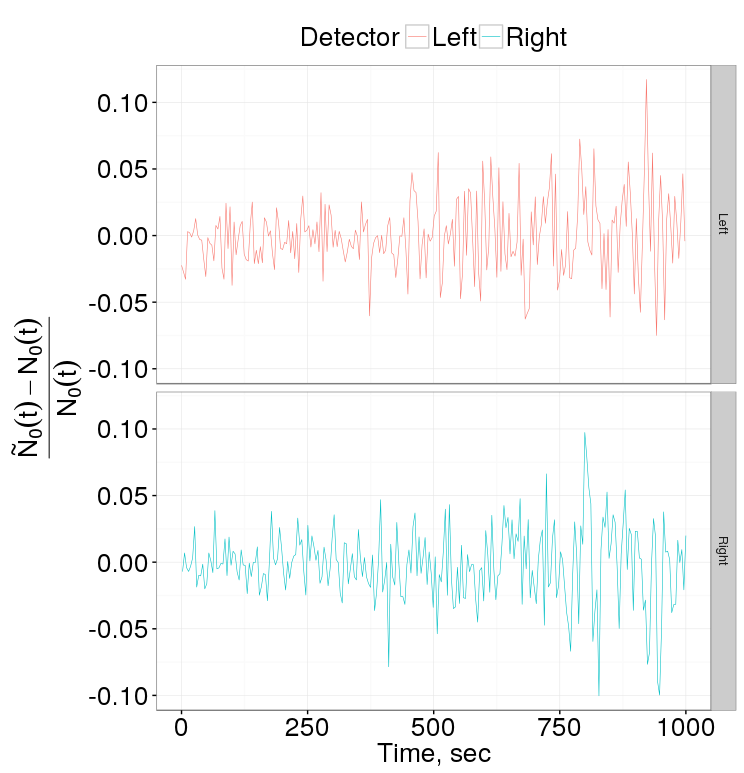
\includegraphics[width=\textwidth]{edm_img/LR_detector_relErr}
	\caption{Относительная ошибка измерения частоты событий на правом и левом
          детекторах как функция времени.\label{fig:LRDetErr}}
\end{figure}

\begin{figure}[H]
	\centering
	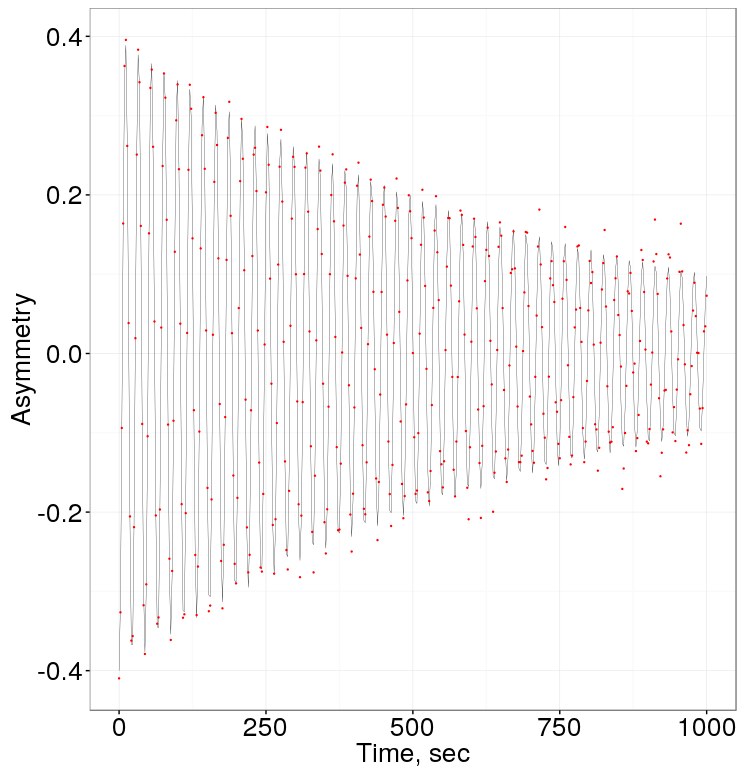
\includegraphics[width=\textwidth]{edm_img/Asymmetry}
	\caption{Ожидание (чёрная линия) и измерения (красные точки)
          асимметрии сечения.\label{fig:Asym}}
\end{figure}

\section{Угловая скорость паразитной МДМ прецессии}
На Рисунке~\ref{fig:Linearity_test_shifting_gauss} представлена ожидаемая частота прецессии поляризации пучка (засчёт МДМ) в зависимости от среднего угла наклона спин-ротаторов. Ожидаемая дисперсия углов наклонов элементов находится в районе $10^{-4}$ радиан. Как видно из рисунка, при величина угловой скорости МДМ прецессии при этом слишком велика, чтобы наблюдать медленное ЭДМ-нарастание вертикальной компоненты поляризации, как предложено в~\cite{BNL:Deuteron2008}.
\begin{figure}[H]
  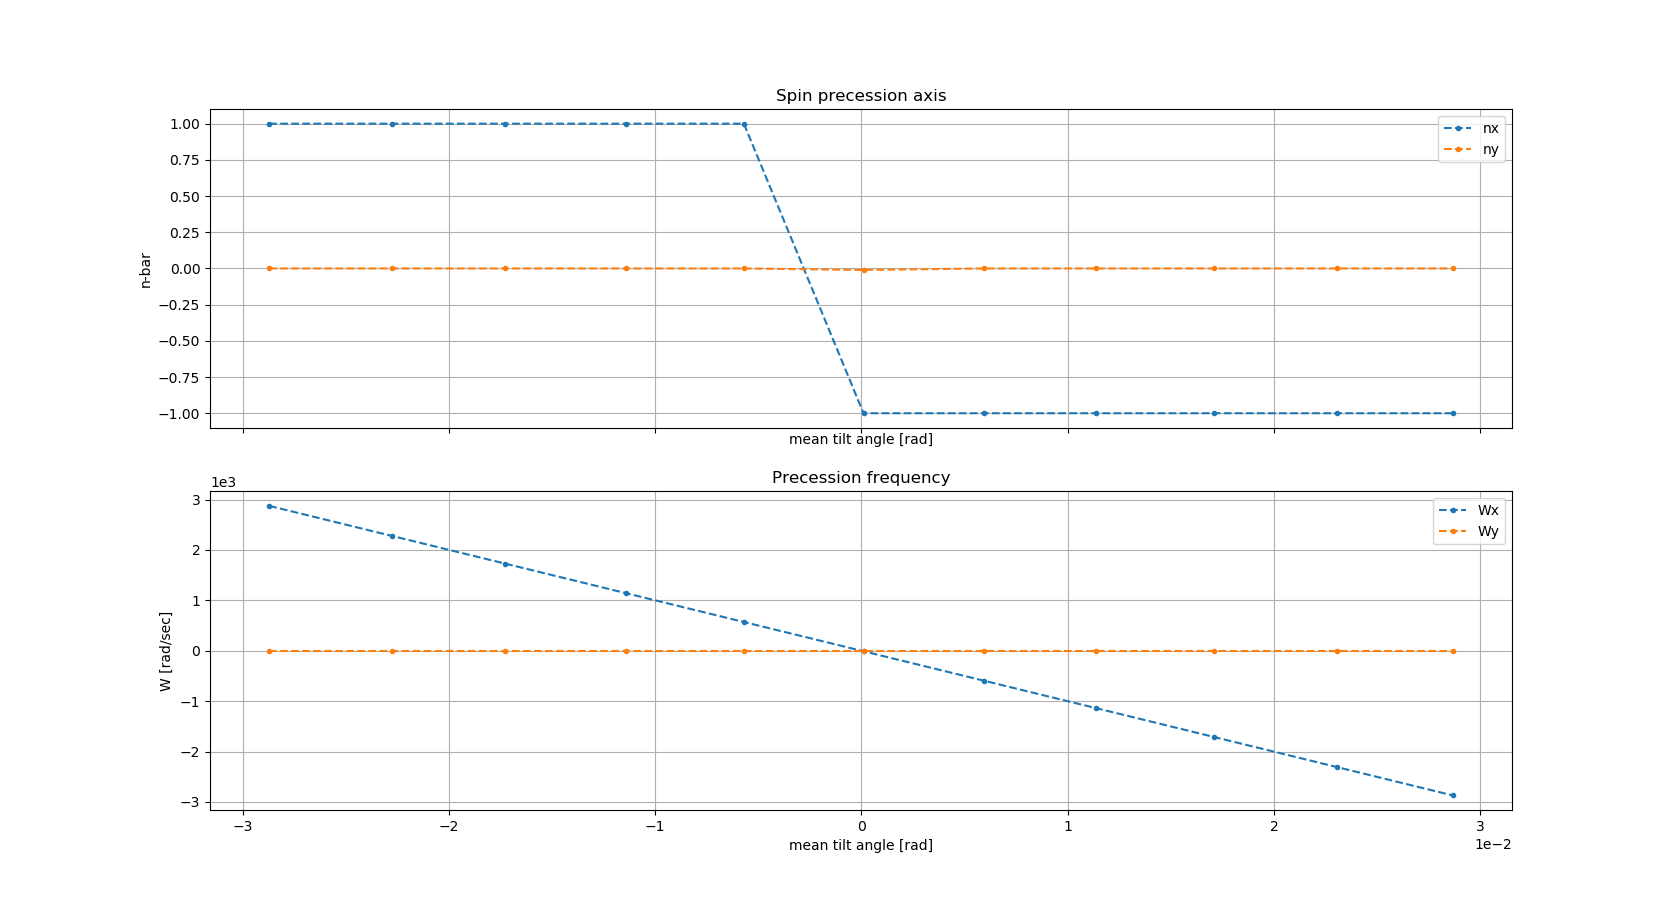
\includegraphics[width=\textwidth]{edm_img/linearity_test_shifting_gauss}
  \caption{Ось прецессии спина и частоты прецессии для неидеальной FS
    структуры, при наклонах E+B элементов.\label{fig:Linearity_test_shifting_gauss}}
\end{figure}

\chapter{Заключения и выводы}
По результатам проверки теоретической возможности проведения эксперимента по поиску ЭДМ дейтрона методом Frequency Domain, были сделаны следующие наблюдения:
\begin{enumerate}
\item обоснованная длительность цикла измерений находится в диапазоне от двух до трёх постоянных времени жизни поляризации $\LTd$;
\item при этом, статистически нет препятствий получению верхнего предела оценки ЭДМ дейтрона на уровне $10^{-29}~e\cdot cm$ за полное время измерений в один год;
\item скорость паразитного МДМ вращения линейно зависит от среднего угла наклона спин-ротаторов, и не зависит от конкретной реализации распределения наклонов;
\item при этом, величина этой скорости достаточно велика, чтобы сделать непрактичным оригинальный FS метод измерения ЭДМ;
\item возможно использование секступольных полей для подавления декогеренции спина и, соответственно, увеличения времени жизни поляризации $\LTd$;
\item использование секступольных полей одновременно выравнивает как скорости вращения спин-векторов частиц вокруг их собственных осей прецессии спина, так и направления самих этих осей, в некоторой области вокруг референсной орбиты;
\item \emph{среднее} (по времени) направление оси прецессии спина частицы зависит от \emph{амплитуды} бетатронных колебаний, но не от конкретного положения частицы в поперечной плоскости вакуумной камеры.
\end{enumerate}

А также выводы:
\begin{enumerate}
  \item Показана возможность улучшения оценки частоты прецессии спина засчёт применения модулированной схемы измерения поляризации.

\item Показана невозможность использования оригинального BNL FS метода измерения ЭДМ дейтрона в накопительном кольце с реалистичной (ожидание среднего угла наклона элементов на уровне $10^{-4}$ радиан) ошибкой установки элементов в связи с величиной угловой скорости МДМ прецессии (см. Рисунок~\ref{fig:Linearity_test_shifting_gauss}).

\item Показана возможность подавления параболической зависимости спин-тюна (и компонент оси прецессии спина) от смещения частицы от референсной орбиты (см. Рисунок~\ref{fig:DECOH_GSY_variation}).
\end{enumerate}


\bibliography{\home/REPOS/EDM/Reports/PhD/PhDRefs}
\bibliographystyle{vancouver}

\end{document}
